% The evaluation loop that isolates the advantage of prediction (P1 analog: fig_architectures).
% Purely structural (no counts): shows where a benchmark must run BOTH a direct-VLA policy and a
% world-model policy under one closed loop, and where the per-capability advantage is measured.
\begin{figure}[t]
\centering
% Hand-drawn (author-illustrated) rendition; replaces the earlier TikZ schematic.
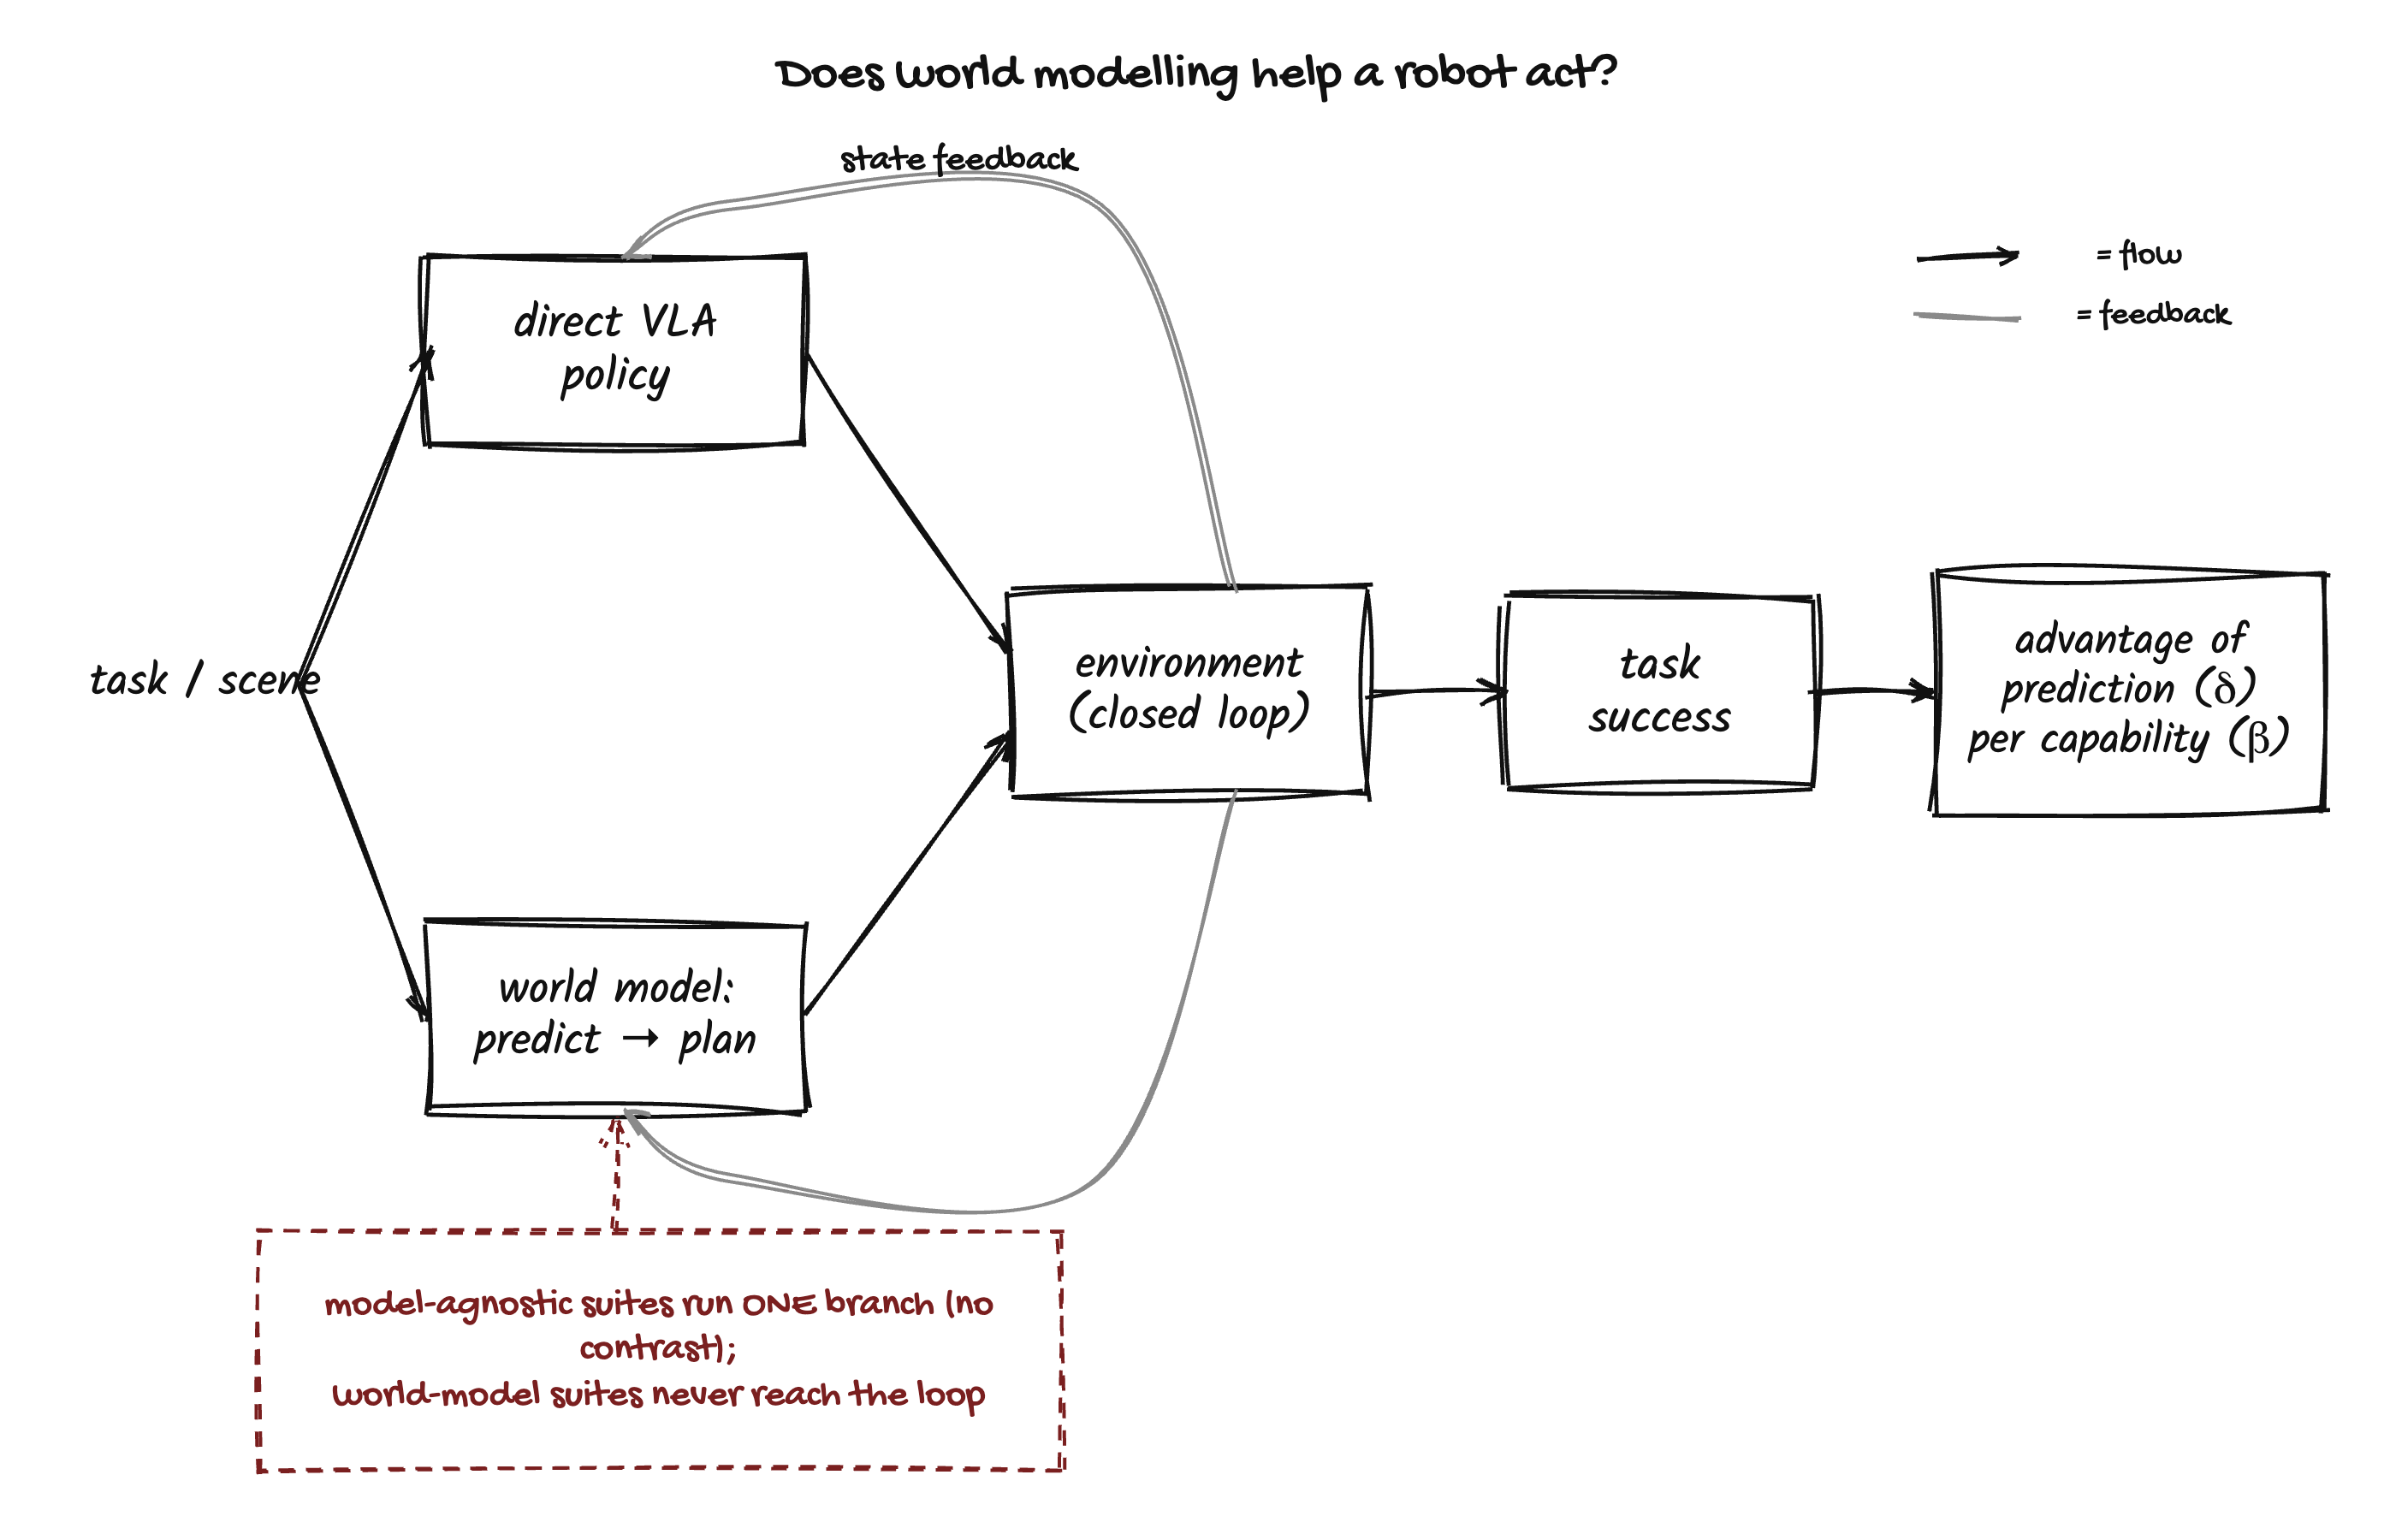
\includegraphics[width=\textwidth]{figures/hand_drawn/fig_eval_loop_hand.png}
\caption{\textbf{The evaluation loop that isolates the advantage of prediction.} A benchmark that
can answer ``does world modelling help a robot act'' must run a direct Vision-Language-Action policy
\emph{and} a world-model policy (predict then plan) under one closed loop, then report the
closed-loop gain ($\delta$) sliced by capability ($\beta$). Today's suites break this loop in one of
two ways: model-agnostic policy suites host a single policy and never build the contrast, while
world-model suites score the prediction open-loop and never execute it (\S\ref{sec:gap}).}
\Description{A left-to-right diagram. A task/scene forks into two branches, a direct VLA policy and a
world model that predicts then plans; both feed an environment closed loop with state feedback,
producing task success, which feeds an advantage-of-prediction measurement sliced per capability. An
annotation notes that model-agnostic suites run only one branch and world-model suites never close
the loop, so the contrast is missing.}
\label{fig:eval_loop}
\end{figure}
